\documentclass{amsart}
\usepackage{graphicx}
\graphicspath{{./}}
\usepackage{hyperref}
\usepackage{csvsimple}
\usepackage{longtable}
\usepackage{epigraph}
\title{Violence Views By Broad Race Worldwide}
\author{Zulfikar Moinuddin Ahmed}
\date{\today}
\begin{document}
\maketitle

\section{Log-Violence Percentage by Race}

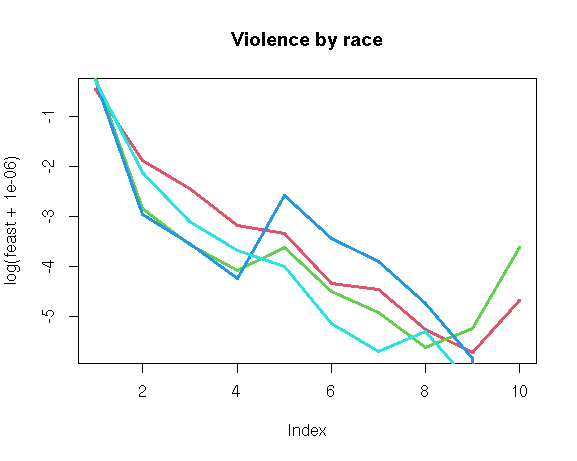
\includegraphics[scale=0.8]{vrace.jpeg}

The red is Far Eastern (Chinese, Japanese, etc). Green is White.  Dark Blue is Black.  Light Blue is Arab/Central Asian.

\section{Differences Are Subtle}

The logarithm graph shows differences that are difficult to detect in the percentage graph, where the exponential model gives indistinguishability.  This is the first observation.  Fine tuned differences in the distribution exist and worth understanding but they will not have a gigantic effect on exponential models.

\end{document}
